\section{Clustering} \label{sec:Clustering}

\blindtext

\subsection{Clustering Results}

\begin{figure}
    \centering
    %\begin{adjustbox}{minipage=\dimexpr\textwidth-2\fboxsep-2\fboxrule,fbox}
    \begin{subfigure}[b]{0.475\textwidth}
        \caption[Kneedle Algorithm]{\textbf{Kneedle Algorithm}}
        \label{subfig:PCA_Cluster_Knee_Kneedle_4}            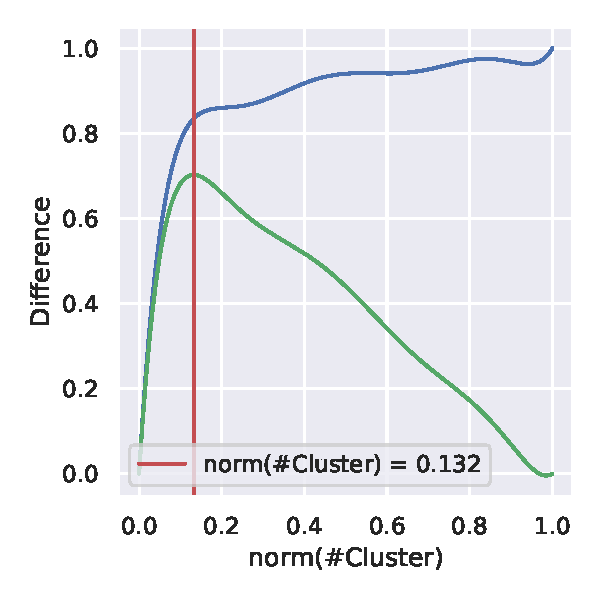
\includegraphics[width=\textwidth]{PCA/Cluster_Knee_Segment_4.pdf}
    \end{subfigure}
    \hfill
    \begin{subfigure}[b]{0.475\textwidth}
        \caption[Kneedle Knee]{\textbf{Kneedle Knee}}
        \label{subfig:PCA_Cluster_Knee_Elbow_4}            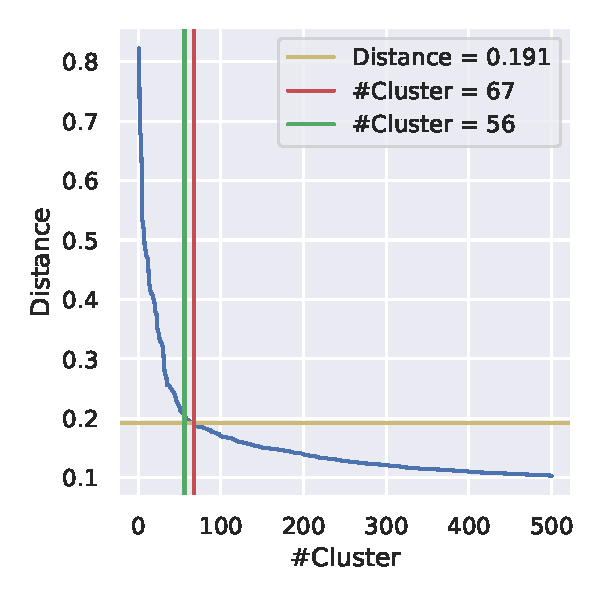
\includegraphics[width=\textwidth]{PCA/Cluster_Elbow_Knee_Segment_4.pdf}
    \end{subfigure}
    \vskip\baselineskip
    \begin{subfigure}[b]{0.475\textwidth}
        \caption[Cluster Distribution]{\textbf{Cluster Distribution}}
        \label{subfig:PCA_Cluster_Kne_Distributione_4}            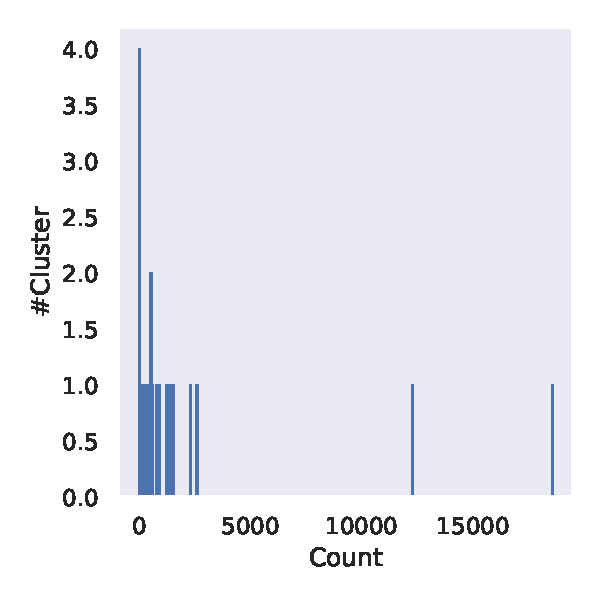
\includegraphics[width=\textwidth]{PCA/Cluster_Distribution_Segment_4.pdf}
    \end{subfigure}
    \hfill
    \begin{subfigure}[b]{0.475\textwidth}
        \caption[Logarithmic Distribution]{\textbf{Logarithmic Distribution}}
        \label{subfig:PCA_Cluster_Knee_Distribution_log_4}            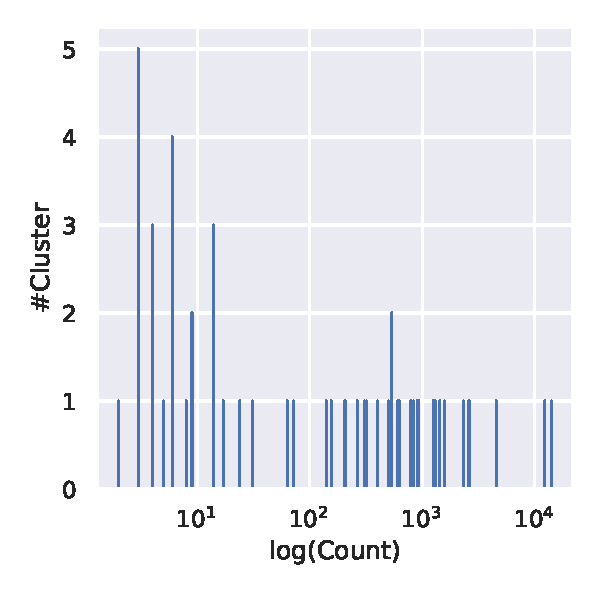
\includegraphics[width=\textwidth]{PCA/Cluster_Distribution_Log_Segment_4.pdf}
    \end{subfigure}
    %\end{adjustbox}
    \caption[Knee based Segment 4 Clustering (\Acrshort{PCA})]{\textbf{Knee based Segment 4 Clustering (\Acrshort{PCA}).}.}
    \label{fig:PCA_Cluster_Knee_4}
\end{figure}

\begin{figure}
    \centering
    %\begin{adjustbox}{minipage=\dimexpr\textwidth-2\fboxsep-2\fboxrule,fbox}
    \begin{subfigure}[b]{0.475\textwidth}
        \caption[\Acrshort{DBCV} Exploration]{\textbf{\Acrshort{DBCV} Exploration}}
        \label{subfig:PCA_Cluster_DBCV_Explo_4}            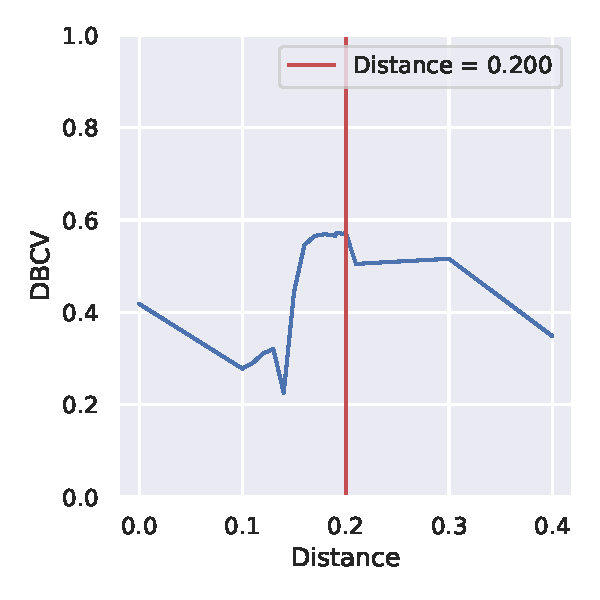
\includegraphics[width=\textwidth]{PCA/Cluster_DBCV_Segment_4.pdf}
    \end{subfigure}
    \hfill
    \begin{subfigure}[b]{0.475\textwidth}
        \caption[\Acrshort{DBCV} Knee]{\textbf{\Acrshort{DBCV} Knee}}
        \label{subfig:PCA_Cluster_DBCV_Elbow_4}            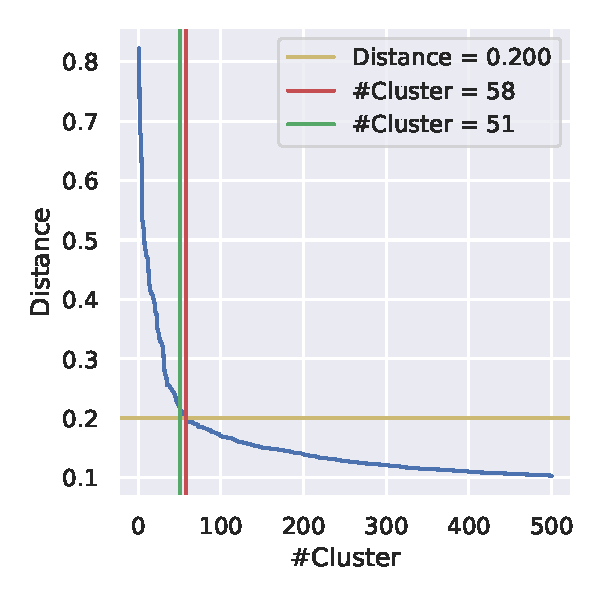
\includegraphics[width=\textwidth]{PCA/Cluster_Elbow_DBCV_Segment_4.pdf}
    \end{subfigure}
    \vskip\baselineskip
    \begin{subfigure}[b]{0.475\textwidth}
        \caption[Cluster Distribution]{\textbf{Cluster Distribution}}
        \label{subfig:PCA_Cluster_DBCV_Distribution_4}            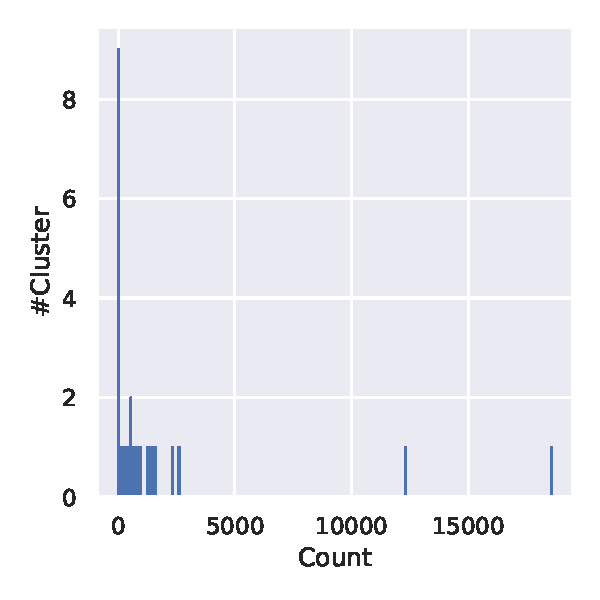
\includegraphics[width=\textwidth]{PCA/Cluster_Distribution_Segment_4_alternative.pdf}
    \end{subfigure}
    \hfill
    \begin{subfigure}[b]{0.475\textwidth}
        \caption[Logarithmic Distribution]{\textbf{Logarithmic Distribution}}
        \label{subfig:PCA_Cluster_DBCV_Distribution_log_4}            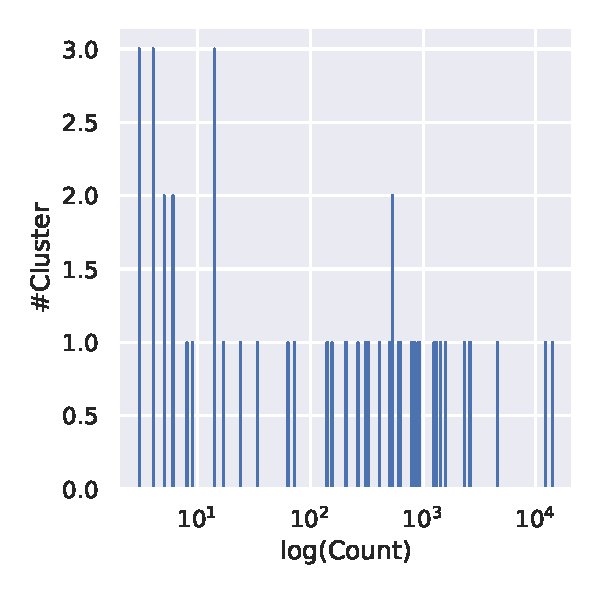
\includegraphics[width=\textwidth]{PCA/Cluster_Distribution_Log_Segment_4_alternative.pdf}
    \end{subfigure}
    %\end{adjustbox}
    \caption[\Acrshort{DBCV} based Segment 4 Clustering (\Acrshort{PCA})]{\textbf{\Acrshort{DBCV} based Segment 4 Clustering (\Acrshort{PCA}).}.}
    \label{fig:PCA_Cluster_DBCV_4}
\end{figure}

\begin{figure}
    \centering
    %\begin{adjustbox}{minipage=\dimexpr\textwidth-2\fboxsep-2\fboxrule,fbox}
    \begin{subfigure}[b]{0.475\textwidth}
        \caption[Kneedle Algorithm]{\textbf{Kneedle Algorithm}}
        \label{subfig:UMAP_Cluster_Knee_Kneedle_4}            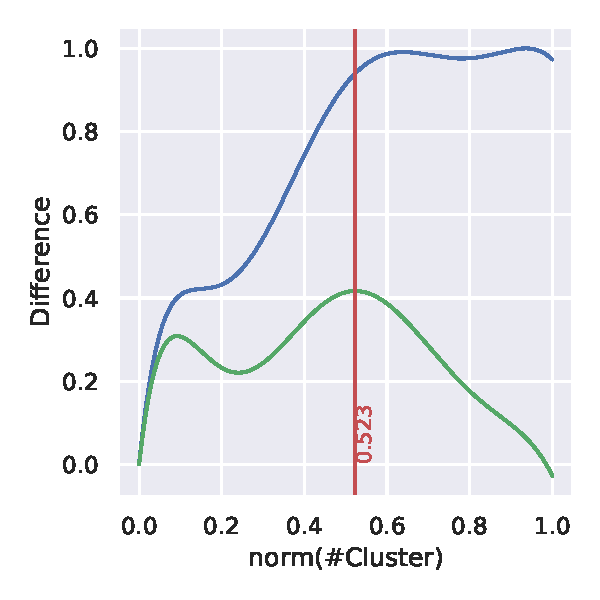
\includegraphics[width=\textwidth]{UMAP/Cluster_Knee_Segment_4.pdf}
    \end{subfigure}
    \hfill
    \begin{subfigure}[b]{0.475\textwidth}
        \caption[Kneedle Knee]{\textbf{Kneedle Knee}}
        \label{subfig:UMAP_Cluster_Knee_Elbow_4}            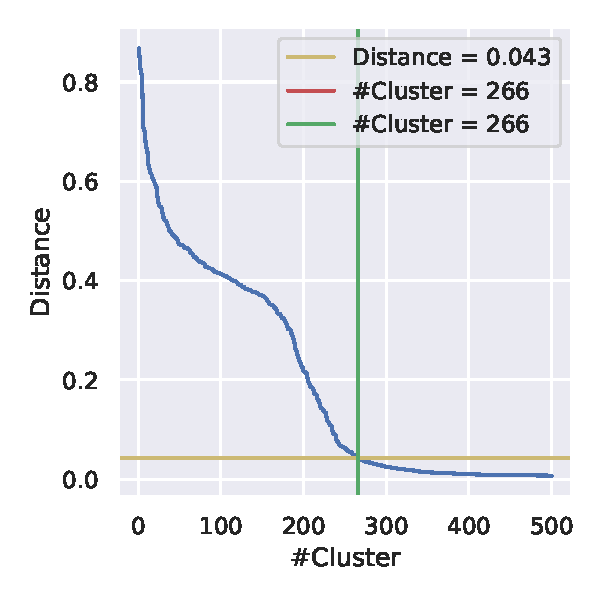
\includegraphics[width=\textwidth]{UMAP/Cluster_Elbow_Knee_Segment_4.pdf}
    \end{subfigure}
    \vskip\baselineskip
    \begin{subfigure}[b]{0.475\textwidth}
        \caption[Cluster Distribution]{\textbf{Cluster Distribution}}
        \label{subfig:UMAP_Cluster_Kne_Distributione_4}            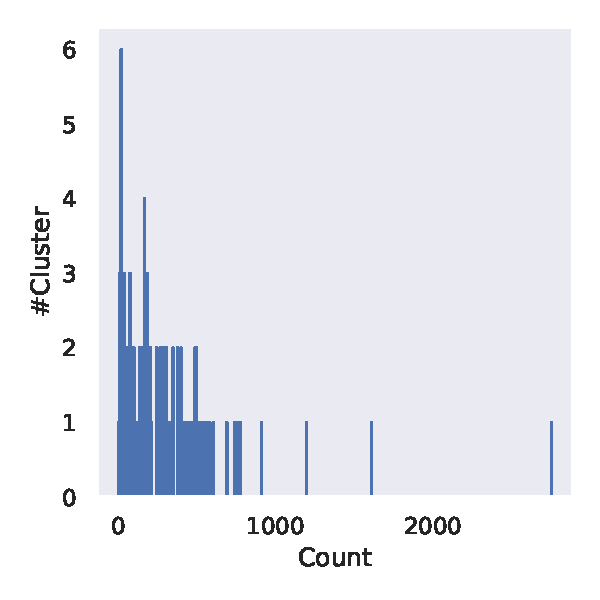
\includegraphics[width=\textwidth]{UMAP/Cluster_Distribution_Segment_4.pdf}
    \end{subfigure}
    \hfill
    \begin{subfigure}[b]{0.475\textwidth}
        \caption[Logarithmic Distribution]{\textbf{Logarithmic Distribution}}
        \label{subfig:UMAP_Cluster_Knee_Distribution_log_4}            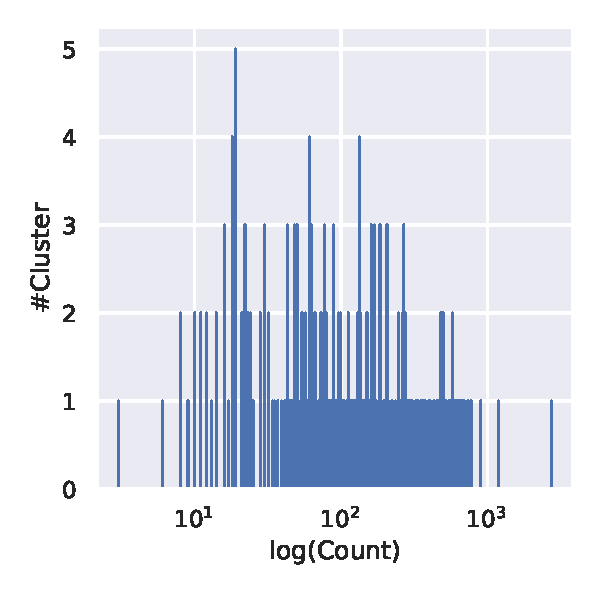
\includegraphics[width=\textwidth]{UMAP/Cluster_Distribution_Log_Segment_4.pdf}
    \end{subfigure}
    %\end{adjustbox}
    \caption[Knee based Segment 4 Clustering (\Acrshort{UMAP})]{\textbf{Knee based Segment 4 Clustering (\Acrshort{UMAP}).}.}
    \label{fig:UMAP_Cluster_Knee_4}
\end{figure}

\begin{figure}
    \centering
    %\begin{adjustbox}{minipage=\dimexpr\textwidth-2\fboxsep-2\fboxrule,fbox}
    \begin{subfigure}[b]{0.475\textwidth}
        \caption[\Acrshort{DBCV} Exploration]{\textbf{\Acrshort{DBCV} Exploration}}
        \label{subfig:UMAP_Cluster_DBCV_Explo_4}            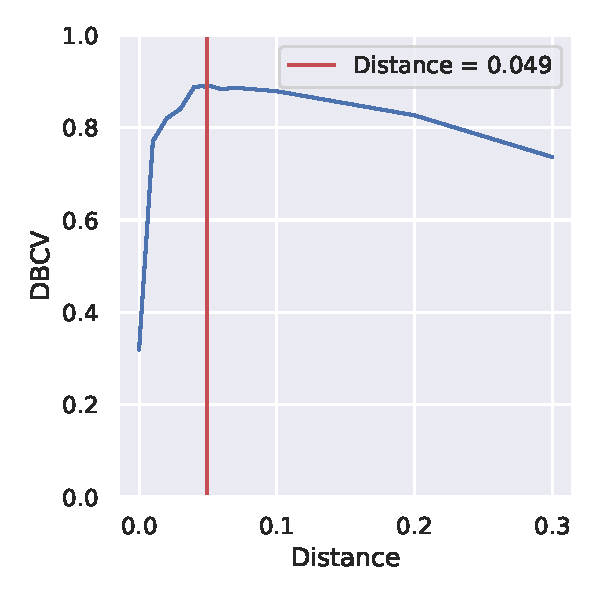
\includegraphics[width=\textwidth]{UMAP/Cluster_DBCV_Segment_4.pdf}
    \end{subfigure}
    \hfill
    \begin{subfigure}[b]{0.475\textwidth}
        \caption[\Acrshort{DBCV} Knee]{\textbf{\Acrshort{DBCV} Knee}}
        \label{subfig:UMAP_Cluster_DBCV_Elbow_4}            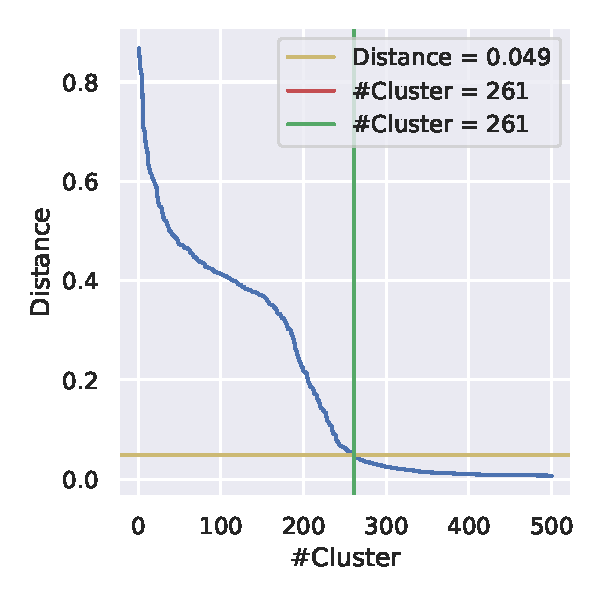
\includegraphics[width=\textwidth]{UMAP/Cluster_Elbow_DBCV_Segment_4.pdf}
    \end{subfigure}
    \vskip\baselineskip
    \begin{subfigure}[b]{0.475\textwidth}
        \caption[Cluster Distribution]{\textbf{Cluster Distribution}}
        \label{subfig:UMAP_Cluster_DBCV_Distribution_4}            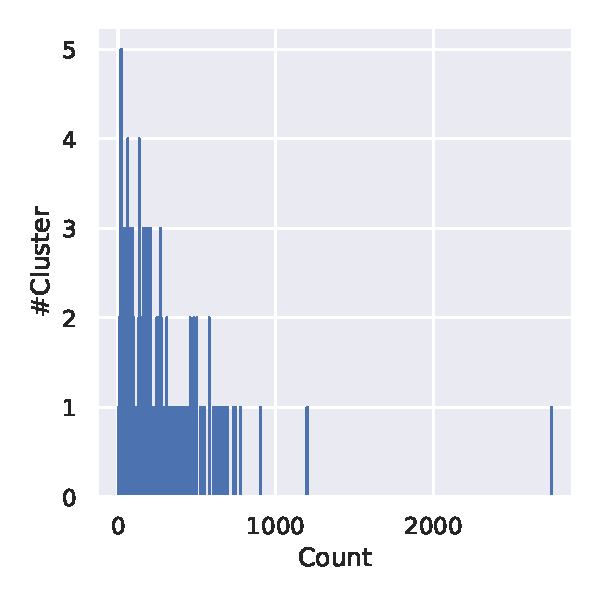
\includegraphics[width=\textwidth]{UMAP/Cluster_Distribution_Segment_4_alternative.pdf}
    \end{subfigure}
    \hfill
    \begin{subfigure}[b]{0.475\textwidth}
        \caption[Logarithmic Distribution]{\textbf{Logarithmic Distribution}}
        \label{subfig:UMAP_Cluster_DBCV_Distribution_log_4}            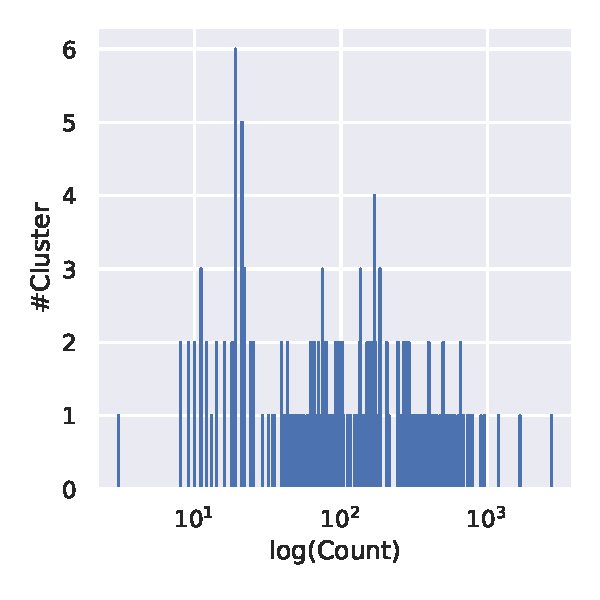
\includegraphics[width=\textwidth]{UMAP/Cluster_Distribution_Log_Segment_4_alternative.pdf}
    \end{subfigure}
    %\end{adjustbox}
    \caption[\Acrshort{DBCV} based Segment 4 Clustering (\Acrshort{UMAP})]{\textbf{\Acrshort{DBCV} based Segment 4 Clustering (\Acrshort{UMAP}).}.}
    \label{fig:UMAP_Cluster_DBCV_4}
\end{figure}

\begin{table}[!hbt]
    \centering
    \caption[Knee based Clustering (\Acrshort{PCA})]{\textbf{Knee based Clustering (\Acrshort{PCA}).}.}
    \label{tab:PCA_Cluster_Knee}
    \pgfplotstabletypeset[
        every head row/.style={
            before row={
                \toprule
                & \multicolumn{3}{l}{\textbf{Cluster}} &  & \multicolumn{2}{l}{\textbf{mixed}} &\\
                \cmidrule(lr){2-4}\cmidrule(lr){6-7}
            },
            after row={
                \midrule
            },
        },
        every last row/.style={
            after row={
                %... & ... & ... & ... & ... & ... & ... & ...\\
                \bottomrule
            },
        },
        begin table=\begin{tabular*}{\textwidth},
        end table=\end{tabular*},
        columns={0,1,2,3,4,5,6,7,8},
        columns/0/.style={int detect, multicolumn names=l,column name=\textbf{Segment}, column type=@{\extracolsep{\fill}\hspace{6pt}}r},
        columns/1/.style={int detect, multicolumn names=l,column name=\textbf{\#Final}, column type=r},
        columns/2/.style={int detect, multicolumn names=l,column name=\textbf{\#Raw}, column type=r},
        columns/3/.style={multicolumn names=l,column name=\textbf{Normalized}, column type=r},
        columns/4/.style={int detect, multicolumn names=l,column name=\textbf{\#Unclustered}, column type=r},
        columns/5/.style={int detect, multicolumn names=l,column name=\textbf{H}, column type=r},
        columns/6/.style={int detect, multicolumn names=l,column name=\textbf{N}, column type=r},
        columns/7/.style={multicolumn names=l,column name=\textbf{Distance}, column type=r},
        columns/8/.style={multicolumn names=l,column name=\textbf{Variance}, column type=r},
    ]
    {PCA/information.csv}
\end{table}

\begin{table}[!hbt]
    \centering
    \caption[\Acrshort{DBCV} based Clustering (\Acrshort{PCA})]{\textbf{\Acrshort{DBCV} based Clustering (\Acrshort{PCA}).}.}
    \label{tab:PCA_Cluster_DBCV}
    \pgfplotstabletypeset[
        every head row/.style={
            before row={
                \toprule
                & \multicolumn{2}{l}{\textbf{Cluster}} &  & \multicolumn{2}{l}{\textbf{mixed}} & &\\
                \cmidrule(lr){2-3}\cmidrule(lr){5-6}
            },
            after row={
                \midrule
            },
        },
        every last row/.style={
            after row={
                %... & ... & ... & ... & ... & ... & ... & ...\\
                \bottomrule
            },
        },
        begin table=\begin{tabular*}{\textwidth},
        end table=\end{tabular*},
        columns={0,1,2,3,4,5,6,7,8},
        columns/0/.style={int detect, multicolumn names=l,column name=\textbf{Segment}, column type=@{\extracolsep{\fill}\hspace{6pt}}r},
        columns/1/.style={int detect, multicolumn names=l,column name=\textbf{\#Final}, column type=r},
        columns/2/.style={int detect, multicolumn names=l,column name=\textbf{\#Raw}, column type=r},
        columns/3/.style={int detect, multicolumn names=l,column name=\textbf{\#Unclustered}, column type=r},
        columns/4/.style={int detect, multicolumn names=l,column name=\textbf{H}, column type=r},
        columns/5/.style={int detect, multicolumn names=l,column name=\textbf{N}, column type=r},
        columns/6/.style={multicolumn names=l,column name=\textbf{Distance}, column type=r},
        columns/7/.style={multicolumn names=l,column name=\textbf{DBCV}, column type=r},
        columns/8/.style={multicolumn names=l,column name=\textbf{Variance}, column type=r},
    ]
    {PCA/information_alt.csv}
\end{table}

\begin{table}[!hbt]
    \centering
    \caption[Knee based Clustering (\Acrshort{UMAP})]{\textbf{Knee based Clustering (\Acrshort{UMAP}).}.}
    \label{tab:UMAP_Cluster_Knee}
    \pgfplotstabletypeset[
        every head row/.style={
            before row={
                \toprule
                & \multicolumn{3}{l}{\textbf{Cluster}} &  & \multicolumn{2}{l}{\textbf{mixed}} &\\
                \cmidrule(lr){2-4}\cmidrule(lr){6-7}
            },
            after row={
                \midrule
            },
        },
        every last row/.style={
            after row={
                %... & ... & ... & ... & ... & ... & ... & ...\\
                \bottomrule
            },
        },
        begin table=\begin{tabular*}{\textwidth},
        end table=\end{tabular*},
        columns={0,1,2,3,4,5,6,7,8},
        columns/0/.style={int detect, multicolumn names=l,column name=\textbf{Segment}, column type=@{\extracolsep{\fill}\hspace{6pt}}r},
        columns/1/.style={int detect, multicolumn names=l,column name=\textbf{\#Final}, column type=r},
        columns/2/.style={int detect, multicolumn names=l,column name=\textbf{\#Raw}, column type=r},
        columns/3/.style={multicolumn names=l,column name=\textbf{Normalized}, column type=r},
        columns/4/.style={int detect, multicolumn names=l,column name=\textbf{\#Unclustered}, column type=r},
        columns/5/.style={int detect, multicolumn names=l,column name=\textbf{H}, column type=r},
        columns/6/.style={int detect, multicolumn names=l,column name=\textbf{N}, column type=r},
        columns/7/.style={multicolumn names=l,column name=\textbf{Distance}, column type=r},
        columns/8/.style={multicolumn names=l,column name=\textbf{Variance}, column type=r},
    ]
    {UMAP/information.csv}
\end{table}

\begin{table}[!hbt]
    \centering
    \caption[\Acrshort{DBCV} based Clustering (\Acrshort{UMAP})]{\textbf{\Acrshort{DBCV} based Clustering (\Acrshort{UMAP}).}.}
    \label{tab:UMAP_Cluster_DBCV}
    \pgfplotstabletypeset[
        every head row/.style={
            before row={
                \toprule
                & \multicolumn{2}{l}{\textbf{Cluster}} &  & \multicolumn{2}{l}{\textbf{mixed}} & &\\
                \cmidrule(lr){2-3}\cmidrule(lr){5-6}
            },
            after row={
                \midrule
            },
        },
        every last row/.style={
            after row={
                %... & ... & ... & ... & ... & ... & ... & ...\\
                \bottomrule
            },
        },
        begin table=\begin{tabular*}{\textwidth},
        end table=\end{tabular*},
        columns={0,1,2,3,4,5,6,7,8},
        columns/0/.style={int detect, multicolumn names=l,column name=\textbf{Segment}, column type=@{\extracolsep{\fill}\hspace{6pt}}r},
        columns/1/.style={int detect, multicolumn names=l,column name=\textbf{\#Final}, column type=r},
        columns/2/.style={int detect, multicolumn names=l,column name=\textbf{\#Raw}, column type=r},
        columns/3/.style={int detect, multicolumn names=l,column name=\textbf{\#Unclustered}, column type=r},
        columns/4/.style={int detect, multicolumn names=l,column name=\textbf{H}, column type=r},
        columns/5/.style={int detect, multicolumn names=l,column name=\textbf{N}, column type=r},
        columns/6/.style={multicolumn names=l,column name=\textbf{Distance}, column type=r},
        columns/7/.style={multicolumn names=l,column name=\textbf{DBCV}, column type=r},
        columns/8/.style={multicolumn names=l,column name=\textbf{Variance}, column type=r},
        %row predicate/.code={%
        %    \ifnum#1>0\relax
        %        \ifnum#1<2\relax
        %            \pgfplotstableuserowfalse
        %        \fi
        %    \fi
        %}
    ]
    {UMAP/information_alt.csv}
\end{table}

\blindtext

\subsection{Clustertrees}

\begin{figure}[!hbt]
    \centering
    \begin{tikzpicture}
        \node[anchor=south west,inner sep=0] (image) at (0,0) {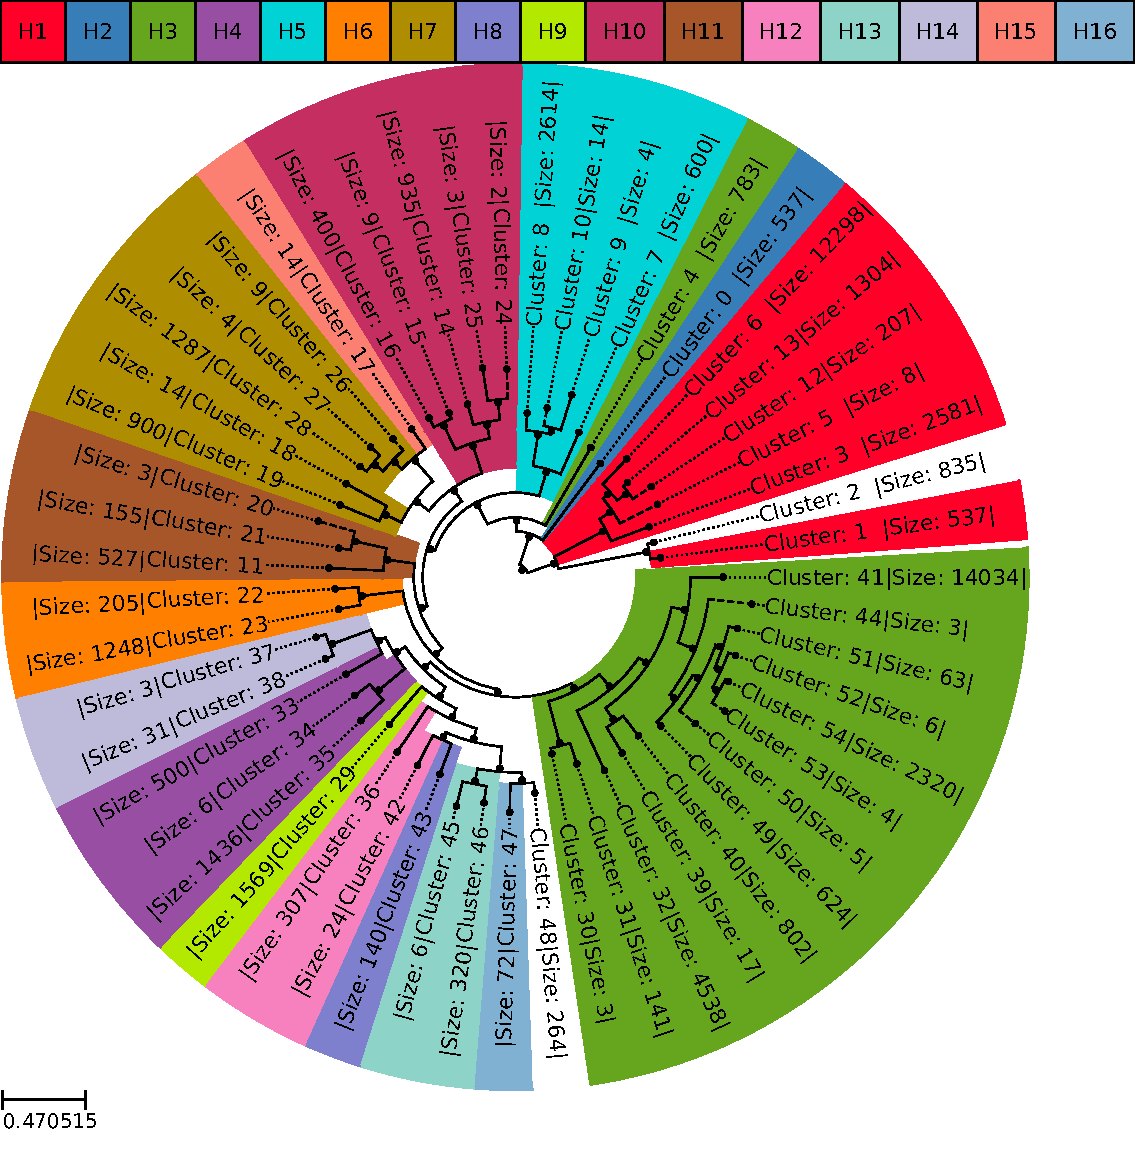
\includegraphics[width=\textwidth]{PCA/Clustertree_Segment_4_H_Knee.pdf}};
        \begin{scope}[x={(image.south east)},y={(image.north west)}]
            %\draw[help lines,xstep=.1,ystep=.1] (0,0) grid (1,1);
            %\draw[black, thick,rounded corners] (7.5,5.3) rectangle (9.4,6.2);
        \end{scope}
    \end{tikzpicture}

    \caption[Knee based Segment 4 Clustertree (\Acrshort{PCA})]{\textbf{Knee based Segment 4 Clustertree (\Acrshort{PCA}).} .}
    \label{fig:PCA_Clusteree_Knee_4}
\end{figure}

\begin{figure}[!hbt]
    \centering
    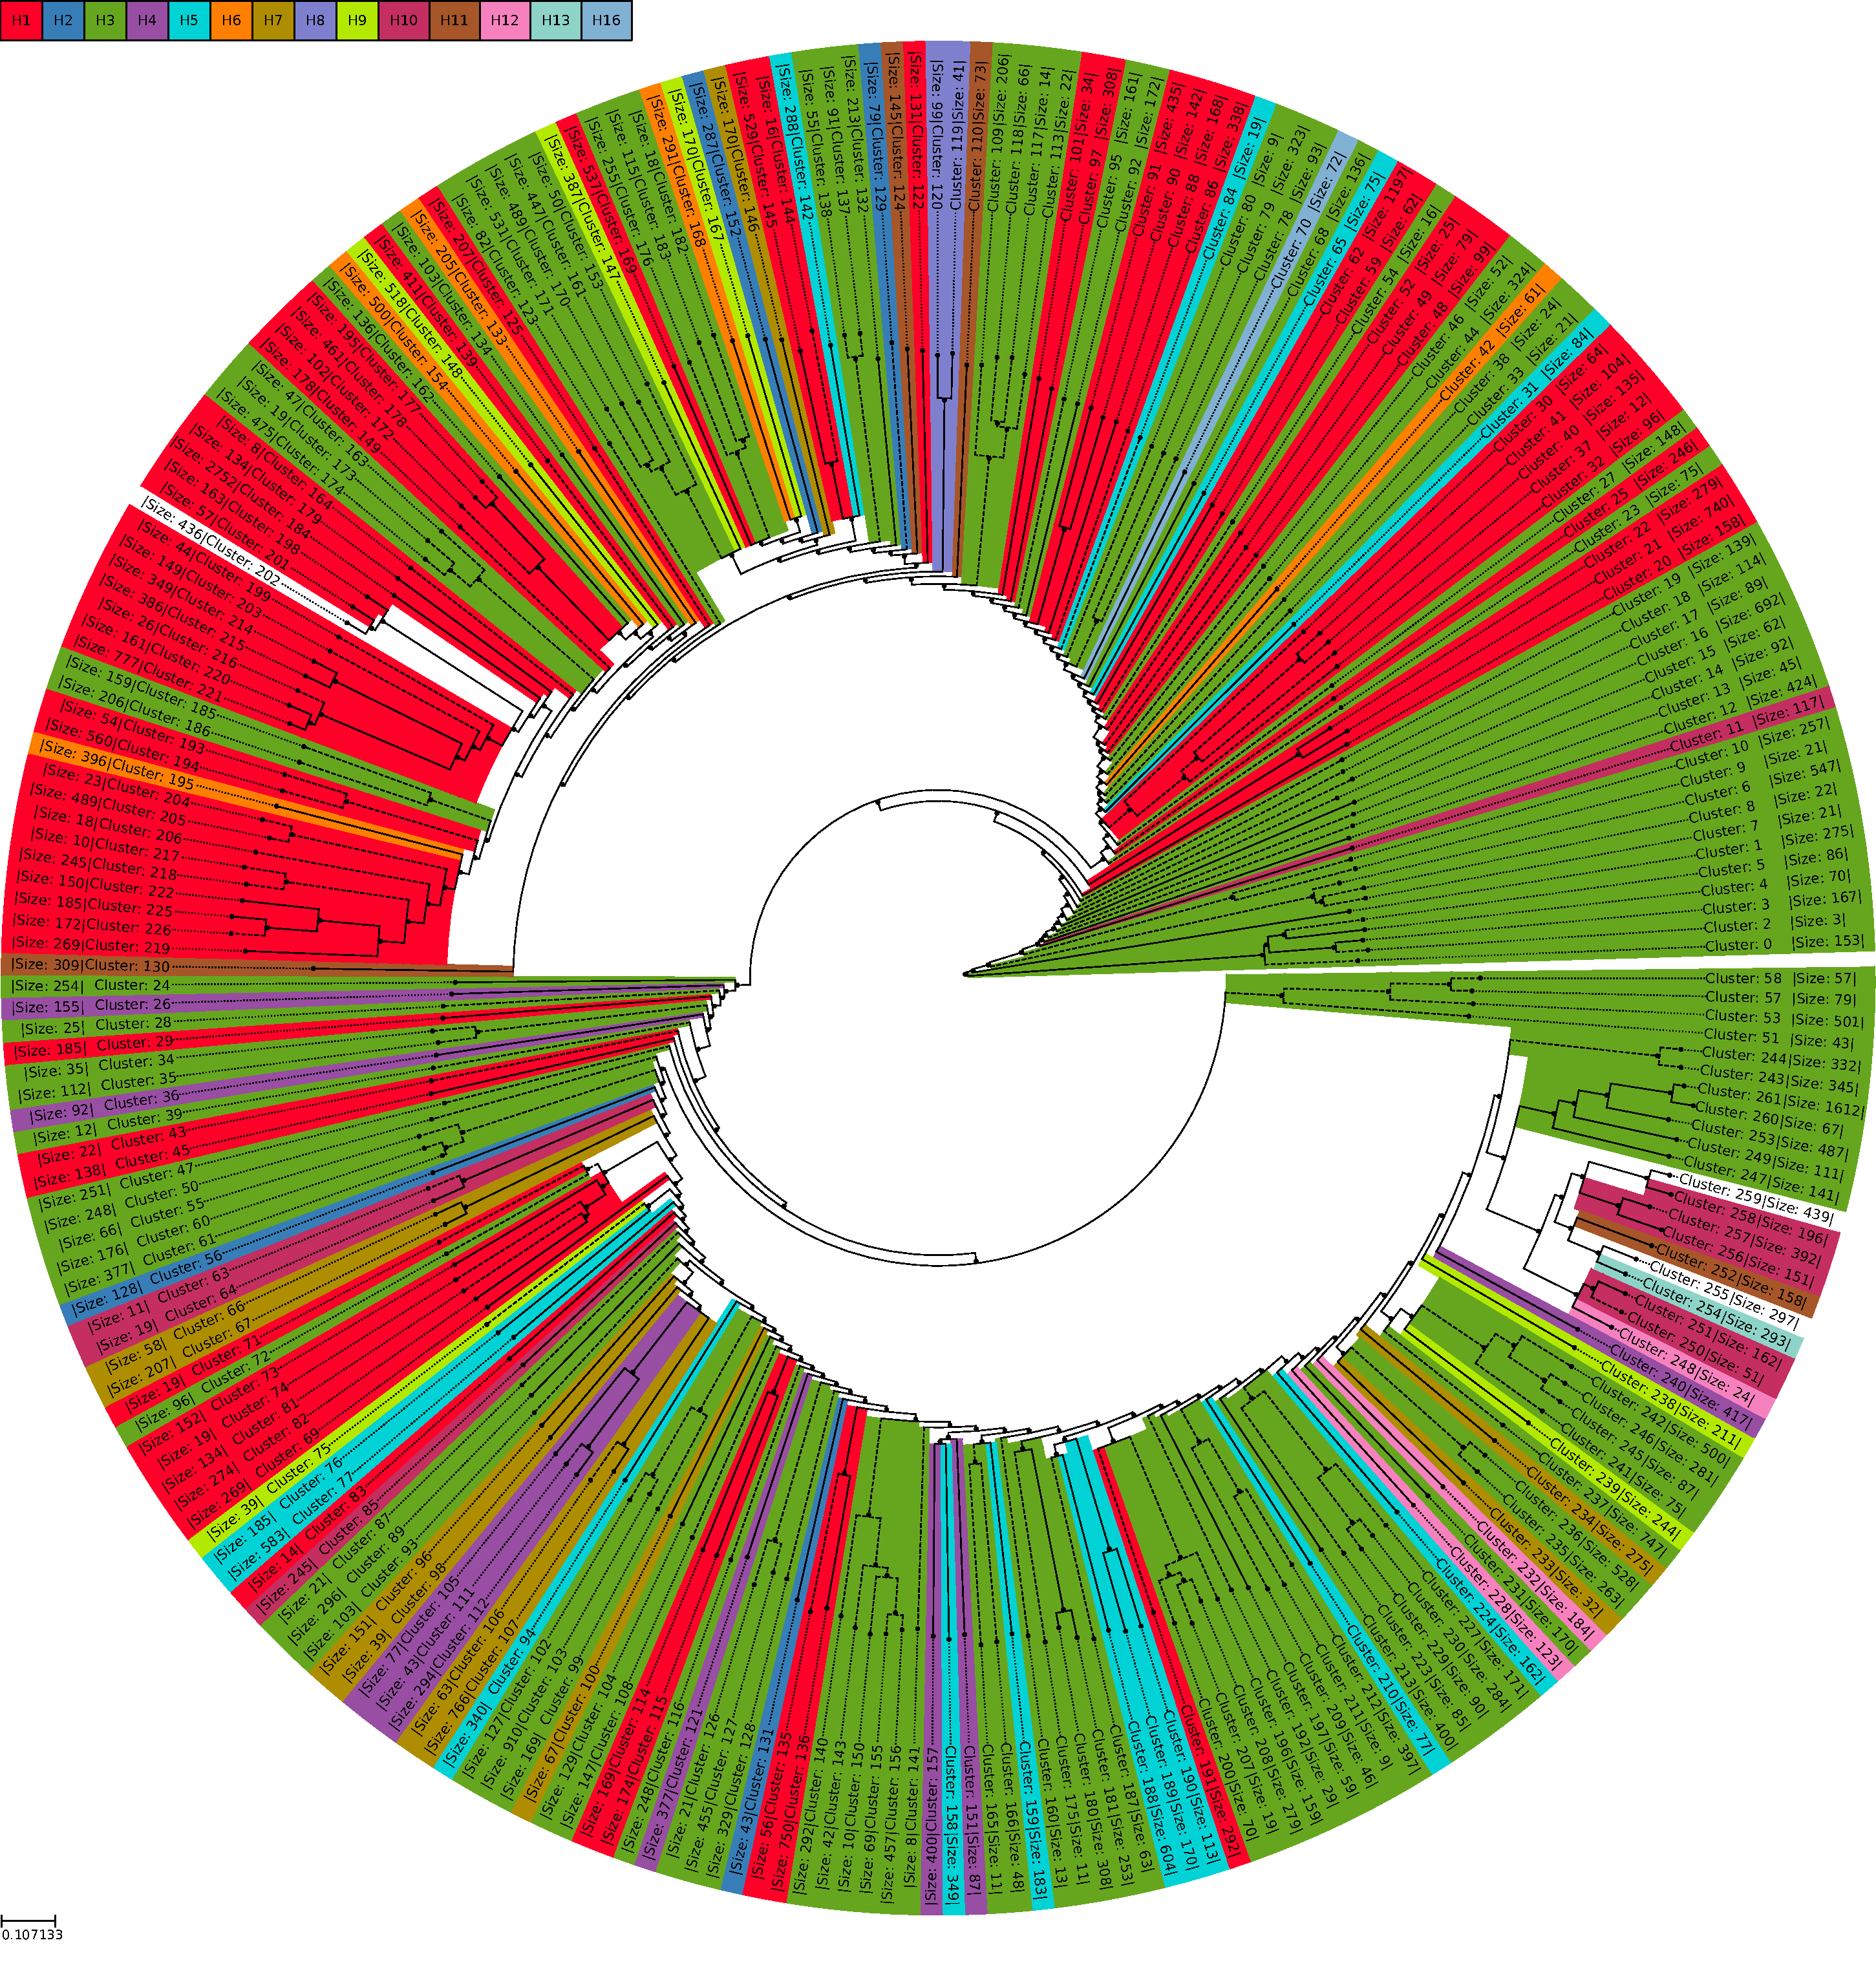
\includegraphics[width=\textwidth]{UMAP/Clustertree_Segment_4_H_Knee.pdf}
    \caption[Knee based Segment 4 Clustertree (\Acrshort{UMAP})]{\textbf{Knee based Segment 4 Clustertree (\Acrshort{UMAP}).} .}
    \label{fig:UMAP_Clusteree_Knee_4}
\end{figure}